
\documentclass[12pt]{article}
\usepackage{setspace}
\usepackage{graphicx}


\usepackage[margin=1in]{geometry}


\setlength\parindent{0pt}
\begin{document}
\begin{titlepage}
\begin{center}
	\Huge
	\textbf{A comparative analysis of Bluetooth based Indoor Localization Systems} \\
	\large    

	\vspace{0.5cm}
	By Sriram Venkatesh\\
	Victoria University of Wellington\\
	300236116 \\

	\vspace{0.9cm}
	\textbf{Abstract}
\end{center}
\doublespacing
	There is an increasing demand for accurate indoor positioning system as the popularity of sensor enabled smartphones rises. However, Indoor Position systems has not yet achieved the same success as that of outdoor positioning. An accurate indoor localization system can be characterized by high accuracy, short training phase, cost-effective and robustness. Accurate indoor localization has the potential to transform the way people navigate indoors in a similar way that GPS transformed the way people navigate outdoors. The objective of this project is to compare different Bluetooth based Indoor Localization System that achieve the most accurate position. 


\end{titlepage}

\doublespacing
\section{Introduction}

\subsection{Indoor Positioning}
The usage of localization systems has risen recently due to the widespread adoption of smartphones. Smartphones take advantage of the information that is accessible from the wireless sensors available on mobile devices, which allow indoor positioning systems to accurately locate users or objects. \\

One of the most popular sensors on a mobile device is the GPS receiver \cite{HABITS}. GPS is used for outdoor position determination. The GPS satellites that orbit the earth transmit signals to a GPS receiver. These receivers passively receive satellite signals, they do not transmit and require an unobstructed view of the sky. \cite{active-passive} Because of the line of sight infrastructure of GPS, it does not provide acceptable indoor localization accuracy \cite{fusionmethod}. Due to this fact, indoor position systems do not use satellites, instead these systems rely on nearby anchors or nodes, which either actively locate or passively provide contextual information for devices to get sensed. \\

In recent years, indoor positioning has been studied by many researchers using different technologies as the nodes. Most of these solutions are based on a single technology. Several indoor positioning systems have been developed over the last decade, relying on a wide variety of technologies including WLAN, infrared and ultra-source among others but there are still a few commercial solutions available, and the ones that do exist are often costly and complex to set up. Currently, the choice of technology and positioning technique depends on requirements of the system. For instance, radio frequency based technologies such as IEEE 802.11 are inexpensive to deploy but has lower precision than many other kinds of technologies, whereas a system based on ultrasound has a very high precision but its relatively expensive. \cite{bluetooth-master-thesis}\\

An accurate indoor localization system can be characterized by high accuracy, short training phase, cost-effective and robustness. Accurate indoor localization has the potential to transform the way people navigate indoors in a similar way that GPS transformed the way people navigate outdoors. \\

\subsection{Scope}
This paper will look into existing systems of indoor localization with bluetooth-based technologies and critically evaluate the best system. This paper is therefore not concerned with the development of new position techniques but rather an evaluation and modification of existing ones. At the conclusion of the report will provide a experimental design for a accurate bluetooth based localization system based on comparative analysis. 

\section{Bluetooth}

In recent years, Bluetooth has emerged as a viable choice of technology in indoor positioning systems due to the increase in the number of Bluetooth devices over the last decade. Bluetooth's properties such as low cost and high availability has led to the development of many indoor positioning systems.  An introduction to the Bluetooth technology is given in this section. This section also describes the different localization measures that available for Bluetooth. These measures are analsysed, and one is selected as the best one to use. 

\subsection{Technology overview}
Bluetooth is a wireless technology standard which is used for transmitting data over short distances. It uses a short-wavelength UHF radio waves from 2.4 to 2.485Ghz range, which is within the 2.4 GHz ISM frequency band. Bluetooth was designed for low power consumption and is based on low-cost transceiver microchips. The Bluetooth specification was conceived in 1993 and is now managed by the Bluetooth Special Interest Group (SIG). \\

Before setting up a connection between devices, a device must perform an inquiry in order to discover other devices that within its range, which is a rather lengthy process. During testing, the Samsung Galaxy S4 took up to 10.24 seconds to connect. Any device that is in discoverable mode will then reply by sending back information about itself, such as its name and unique address. The two devices can pair with each other, a process in which they create a common link key which is stored on each devices. \\

As mentioned above, Bluetooth supports low power communication between nodes. Therefore one of its features is power control. This feature allows a transmitter to adjust its strength based on RSSI. This therefore means we are able to change the transmission strength to ensure the received signal strength is within an optimal range for the receiver. The table below gives an overview of the three different power classes which are defined in the Bluetooth specification. \\

\begin{table}[h]
\centering
\begin{tabular}{|c|c|c|}
\hline
\textbf{Power class} & \textbf{Max power output (dBm)} & \textbf{Min power output (dBm)} \\ \hline
1                    & 20                              & 1                               \\ \hline
2                    & 4                               & -6                              \\ \hline
3                    & 0                               & -                               \\ \hline
\end{tabular}
\caption{Power Classes Bluetooth Devices (sourced from the Bluetooth Specfication)}
\label{my-label}
\end{table}

\subsection{Signal Parameters}

The term Bluetooth signal parameters is used to denote all the status parameters. The Host Controller provides three different parameters. These are:

\begin{itemize}
  \item Received Signal Strength Indicator (RSSI) in connected state
  \item Inquiry Result with RSSI
  \item Link Quality (LQ)
  \item Transmit Power Level (TPL)
\end{itemize}

\subsubsection{Inquiry Result with RSSI}
Devices that want to connect using Bluetooth need to establish a connection. The initiating device will first send an inquiry state, which will continuously send inquiry message at random frequencies. During this period the master sends messages at two different frequencies in a timeslot. In the next time slot the master listens for a inquiry response message at the same frequency from the previous timeslot. The master will send inquiry message for 10.24 secs or until the target device has been detected. \\

Devices that want to be discovered are set at inquiry scan state. It will listen for inquiry messages. Once a slave device receives an inquiry message, it responds after a small delay with Frequency Hopping Synchronization packet (FHS). The FHS packet contains a MAC address and other important information. \\

Using the process above, the devices can discover the Bluetooth devices in its range. If it would like to connect to a device it has found, the initiating devices will wait till it receives a FHS packet with the correct unique address, and send an additional message to synchronize both device to establish a connection. When the initiating device receives the packet, it also receives an RSSI value, which depends on the power of the received signal. The Host Command Interface (HCI), allows for querying for both the MAC address and RSSI value of the last received FHS packet via an event called `Inquiry Result with RSSI'. The Bluetooth specification defines the RSSI value for the `Inquiry Result with RSSI' event as the signal strength in dBm. \\

Below is a graph displaying the RSS samples in a 1 minute time period for stationary target and two access points. \\

\begin{figure}[h!]
\centering
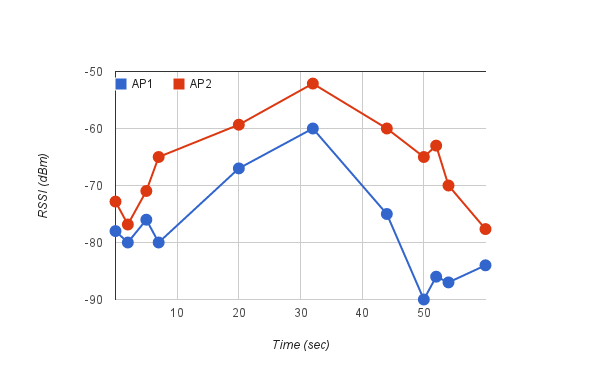
\includegraphics[width=\linewidth]{graph}
\caption{Measured RSS for a stationary target and two access points}
\end{figure} 

We can clearly make two observations in this graph.
\begin{enumerate}
  \item First it displays that for a stationary target, the RSS samples do not form a smooth 
at line but instead show a high variation. For example the difference between the maximum and minimum RSS value for the red line is 20 dBm.
  \item Secondly it shows that the sample rate is low, about 20 samples per minute
\end{enumerate}

The high variation in measurements will affect the localization. Increasing the number of samples can compensate for this effect. However, since the sample rate is low,
relatively large window sizes are required by the localization algorithms to achieve reasonable
accuracy. Real time target tracking is therefore not possible using the inquiry RSSI measure. 


\section{Current Bluetooth localization systems}
The idea of using Bluetooth technology for localization is not novel. Due to the popularity of mobile devices, Bluetooth has become an attractive sensor for localization. This section will describe some of the localization systems and how they work. \\ 

\subsection{Hallberg and Nilsson}
One of the earliest implementations on Bluetooth based localization is that of Hallberg and Nillson. \cite{hallberg-nilsson} They describe, a system which is calibrated using the Log-Normal Shadowing (LNS) model. The log-normal shadowing model attempts to describe signal propagation in buildings and indoor environments. Trilateration was used to estimate target locations. Also in this approach, RSSI values was measured using an active Bluetooth connection which has be proven to be inaccurate. 




\section{Performance Analysis Taxonomy}
The list below gives an overview of the properties which determine the performance of the localization system.

\begin{itemize}
  \item \textbf{Accuracy} is defined as the average distance between the estimated location and the actual location of an object.
  \item \textbf{Responsiveness} The responsiveness determines how quickly the location estimate of a moving target is updated.
  \item \textbf{Calibration effort} is effort required to be calibrate to make location estimates with reasonable accuracy. The amount of effort required for the calibration process can have a big influence on the usefulness of a system, especially if a lot of effort is required. Another factor of the calibration effort is whether it is a process that needs to be performed only once or repetitively. If calibration needs to be performed only once a large effort is less of a problem than if it has to be repeated over time.
  \item \textbf{Adaptiveness} Some changes in the environment may affect the localization system. The ability of the localization system to cope with these changes is called its adaptiveness. 
  \item \textbf{Operational constraints} These define under what circumstances the localization system will provide location estimates with reasonable accuracy
\end{itemize}

An ideal localization system estimates the target location by taking all the above considerations. Unfortunately, these systems do not exist. In reality these systems make a trade-off between these properties, giving more weight for certain properties in certain circumstances. \\

Applying these terminologies, we will compare the several bluetooth based indoor localization techniques.

\section{Critique}


\section{Conclusions}

\bibliographystyle{ieeetr}
\bibliography{bib}
\nocite{*}

\end{document}

